\chapter{Beginning Algebra}

\section{Intro}

This course covers 9th grade math, i.e. the first year of high school mathematics.

\section{Solving Systems of Equations}
% 07 Aug 2025

% \vspace{1 cm}
%
% \centerline{\textbf{\large System of Equations with No Solution or Infinite Solutions}}
%
% \vspace{0.2 cm}

System of Equations can have: một cặp nghiệm (x,y), no Solution or Infinite Solutions.

\vspace{.4cm}

There are three methods for solving systems of Equations:

\begin{enumerate}
  \item Substitution: lấy 1 phương trình dễ tìm x theo y, sau đó thay x vừa tìm vào phương trình còn lại tìm y.
  \item Elimination: cộng hoặc trừ 2 phương trình lại với nhau để khử đi một biến
  \item Graphing
\end{enumerate}

Only Substitution \& Elimination được dùng in the real world. Graphing is really not practical, takes too long, not reliable.

% \begin{equation}
%   \begin{cases}
%     x+4y = 5\\
%     x-4y=-3
%   \end{cases} \iff
%   \begin{cases}
%     x+4y = 5\\
%     x-4y=-3
%   \end{cases} \iff
% \end{equation}

Example of Solving by Elimination (Addition or Subtraction)

% `\right.` is a "phantom" right delimiter
\[
  \begin{aligned}
    &\left\{\begin{aligned} 
      x + 4y &= 5 \\ 
      x - 4y &= -3
    \end{aligned}\right. \iff 
    \left\{\begin{aligned}
      &x +4y = 5\\ 
      &2x = 2
    \end{aligned}\right.
    \\
    \iff &\left\{\begin{aligned} 
      x &= 1 \\ 
      y &= 1
    \end{aligned}\right.
  \end{aligned}
\]

\newpage

Phương pháp elimination, đôi khi phải multiply both equation.

\begin{figure}[htb!]
  \centering
  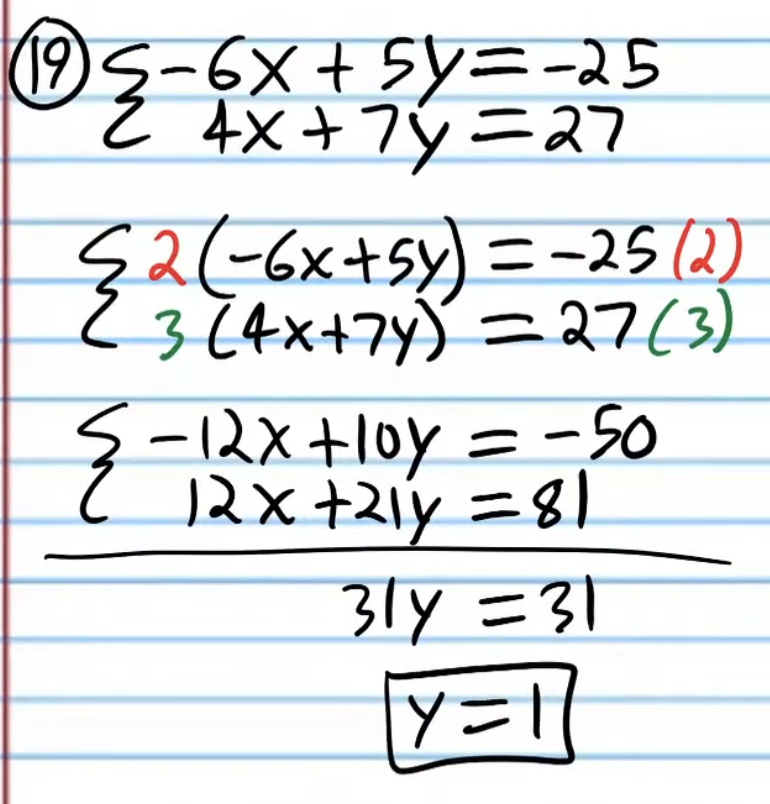
\includegraphics[width=0.4\textwidth]{int0201.png}
  \caption{bài tập}
\end{figure}

Graphical representations of System of Equations.

\begin{figure}[htb!]
  \centering
  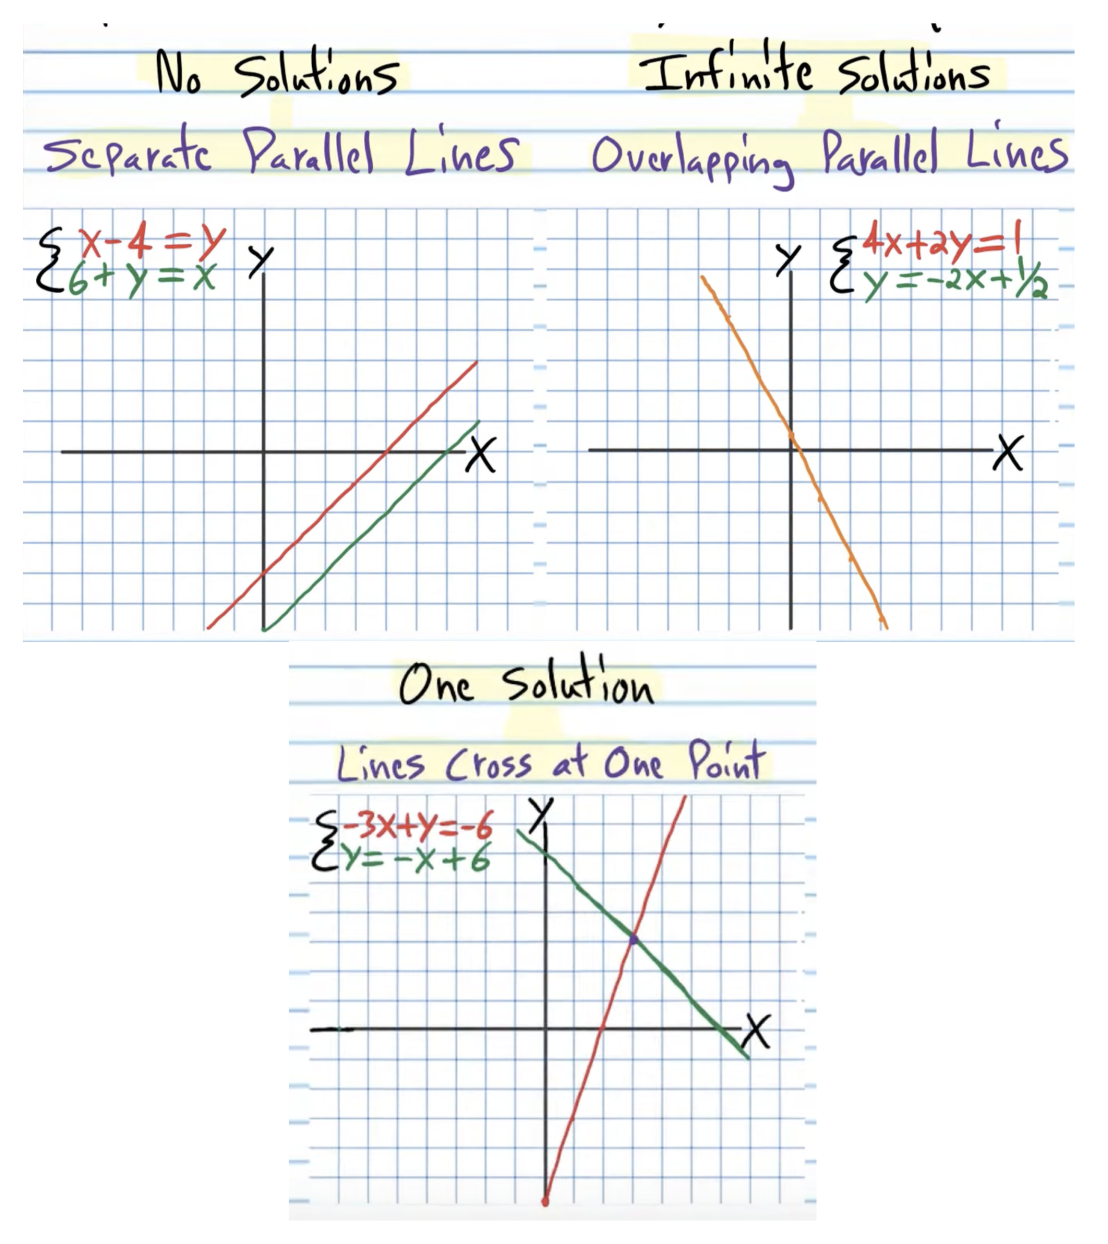
\includegraphics[width=0.6\textwidth]{int0202.png}
  \caption{Graphical representations of sys of Eq}
\end{figure}

\newpage

\section{The Three Forms of Linear Equations and Finding Slope}

% \vspace{1 cm}

% \centerline{\textbf{\large The Slope of a Line}}

% \vspace{0.2 cm}

If \(A(x_{1},y_{1})\text{ and } B(x_{2},y_{2})\) are two points on a line, \textbf{the slope of the line} is defined by the equation below.

\begin{equation}
  m = \frac{y_{2}-y_{1}}{x_{2}-x_{1}}
  \label{eq:3.1}
\end{equation}

\hl{Slope} (hệ số góc) measures the steepness of a line. If the slope of a line is positive, the line travels up moving from left to right. If the slope of a line is negative, the line travels down moving left to right. If the slope of a line is zero, the line is horizontal. If the slope of a line is undefined, the line is vertical.

\textbf{Slope} (hệ số góc) cho biết rate of change. Two parallel lines have \textit{the same} slope.

% \newpage

\begin{figure}[htb!]
  \centering
  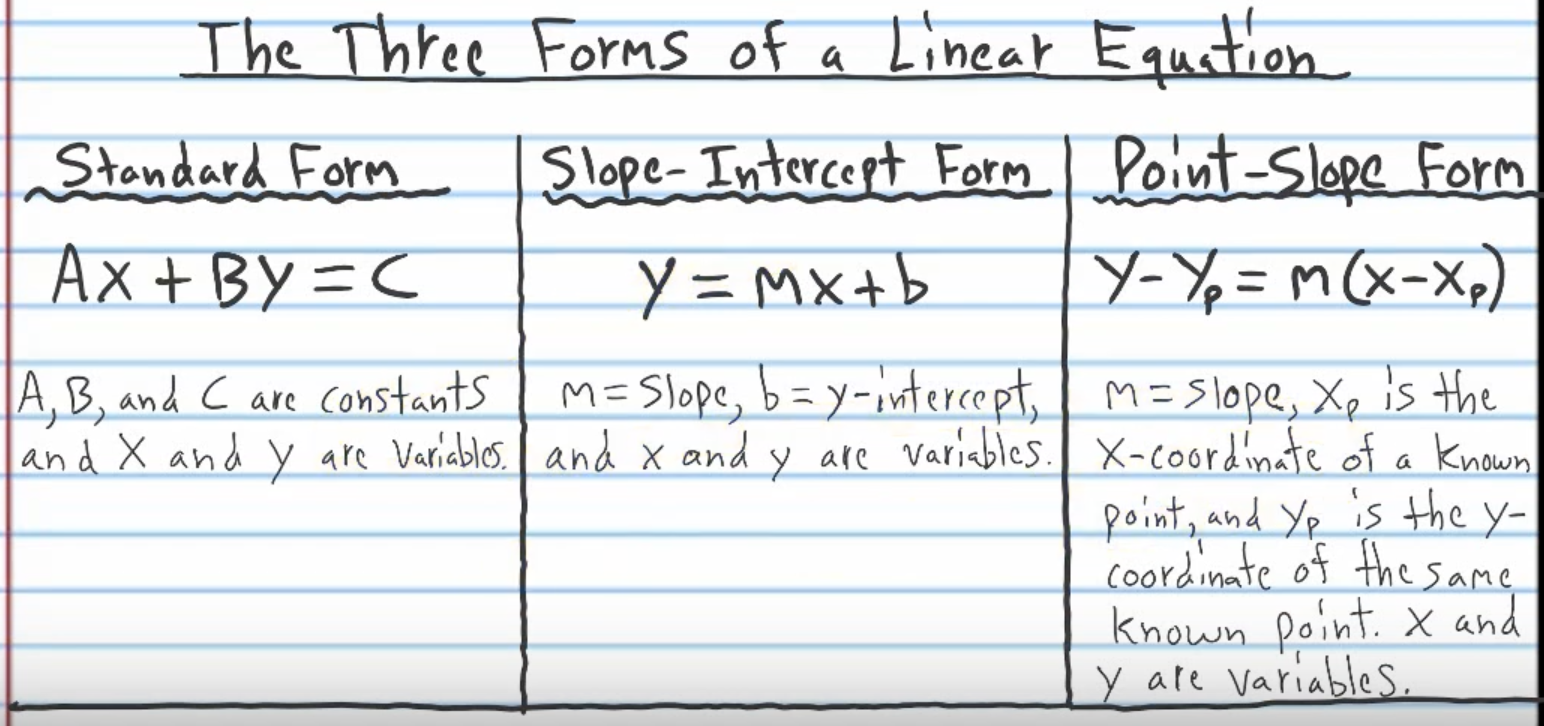
\includegraphics[width=1\textwidth]{beg2601.png}
  \caption{The Three Forms of a Linear Equation}
\end{figure}

% \par\rule{\textwidth}{0.5pt}

% \vspace{1cm}

\textbf{Excercise}: Identify the form of each linear equation below by writing \q{S} for Standard, \q{SI} for slope-intercept, or \q{PS} for point-slope.

$2x+4y=3$: \textbf{S} because the variables x and y are on the same side of the equation.

$4=-8x+7x$: still Standard form, even though the equation is flipped.

$y-4=-3(x-5)$: \textbf{PS}, it is the only form that has parenthesses.

$y=2x+4$: \textbf{SI}, because the y is isolated on one side of the equation.

% \par\rule{\textwidth}{0.5pt}

\vspace{.6cm}

The standard form is not really useful for graphing. Nó không cho biết point, slope or y-intercept. Khi nhìn thấy standard form (x and y on the same side), convert into slope-Intercept form (where y is isolated). Slope-Intercept is the most useful form of the linear equation. Nó cho mình biết slope \& y-intercept.

You also need to be able to convert from Point-slope form to Slope-intercept form. Cách làm cũng là isolate y về một bên.

% Below is not from the course

\vspace{2 cm}

\textbf{Q:} Graph this line \(3x-4y=-6\)

Find the \textbf{x-intercept} by making y = 0. Then find the \textbf{y-intercept} by making x = 0.

\vspace{5mm}

\textbf{Q:} Graph this inequality \(y < -\frac{1}{3}x+2\)

Tìm tọa độ 2 điểm; vẽ đường thẳng.

\begin{itemize}
  \item Nếu \(\le\) thì vẽ straight line and shade under the line.
  \item Nếu > thì vẽ dashed line and shade above the line.
\end{itemize}

\textbf{Q: }Graphing Systems of Inequalities

\vspace{5mm}

Tính \textbf{Distance between 2 points} bằng Eq \ref{eq:3.2} below:

\begin{equation}
  d = \sqrt{(x_{1}-x_{2})^{2} + (y_{1}-y_{2})^{2}}
  \label{eq:3.2}
\end{equation}

\section{Graphing Linear Equations}

\hl{Method 01}: Finding two random points.

\hl{Method 02}: Finding x and y intercepts. Làm giống method 01 nhưng must chose $x=0$ and $y=0$. Useful when dealing with standard form.

% \vspace{4cm}

\hl{Method 03}: Convert to Slope-Intercept form and use slope and y-intercept.

The slope is $\frac{\text{rise}}{\text{run}}$. In the figure below, first we find that the y-intercept is $(0,-1)$. Then we rise up two and run to the right 3 to get to the second point of $(3,1)$.

\begin{figure}[htb!]
  \centering
  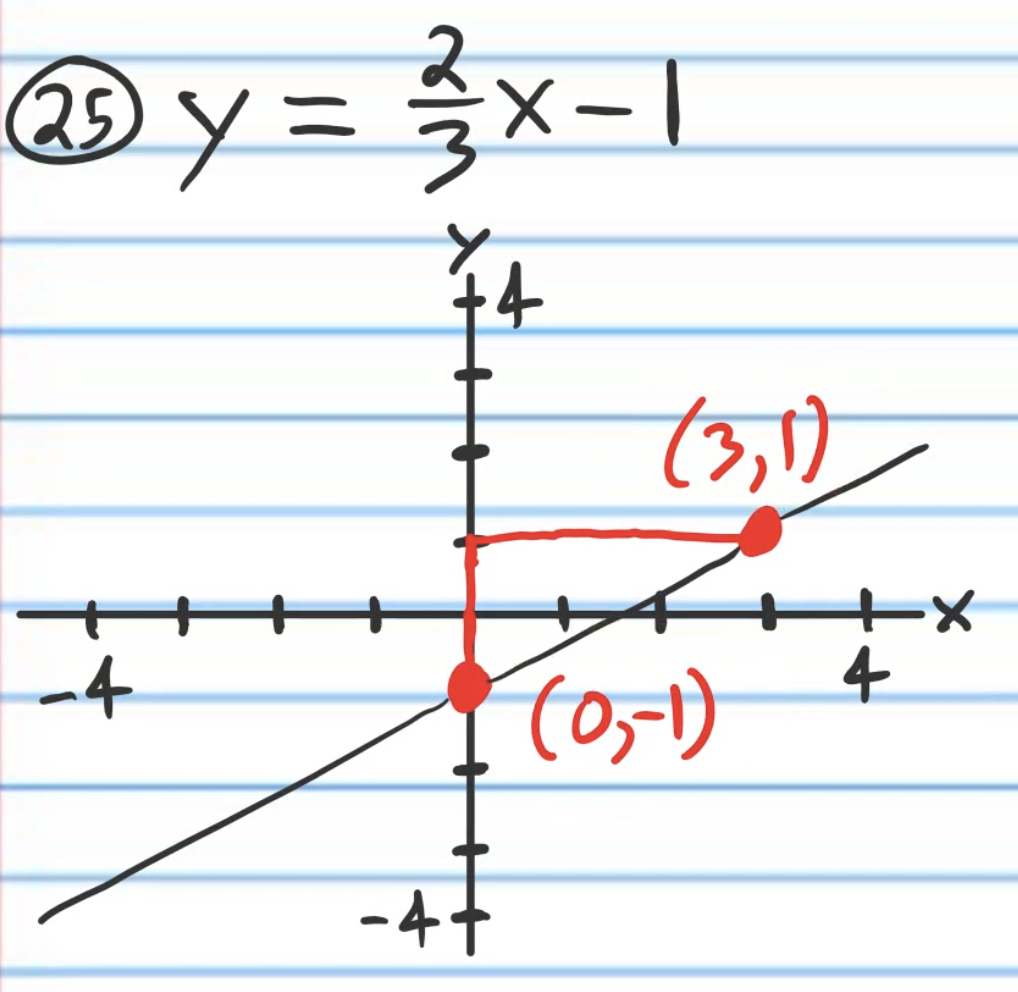
\includegraphics[width=0.5\textwidth]{beg2701.png}
  \caption{The slope is rise/run}
\end{figure}

\newpage

When the slope is a negative number, instead of rising up, we go down and to the right. In the figure below, we go down 4 and then go 5 to the right (một ô đơn vị ứng với 2 units).

\begin{figure}[htb!]
  \centering
  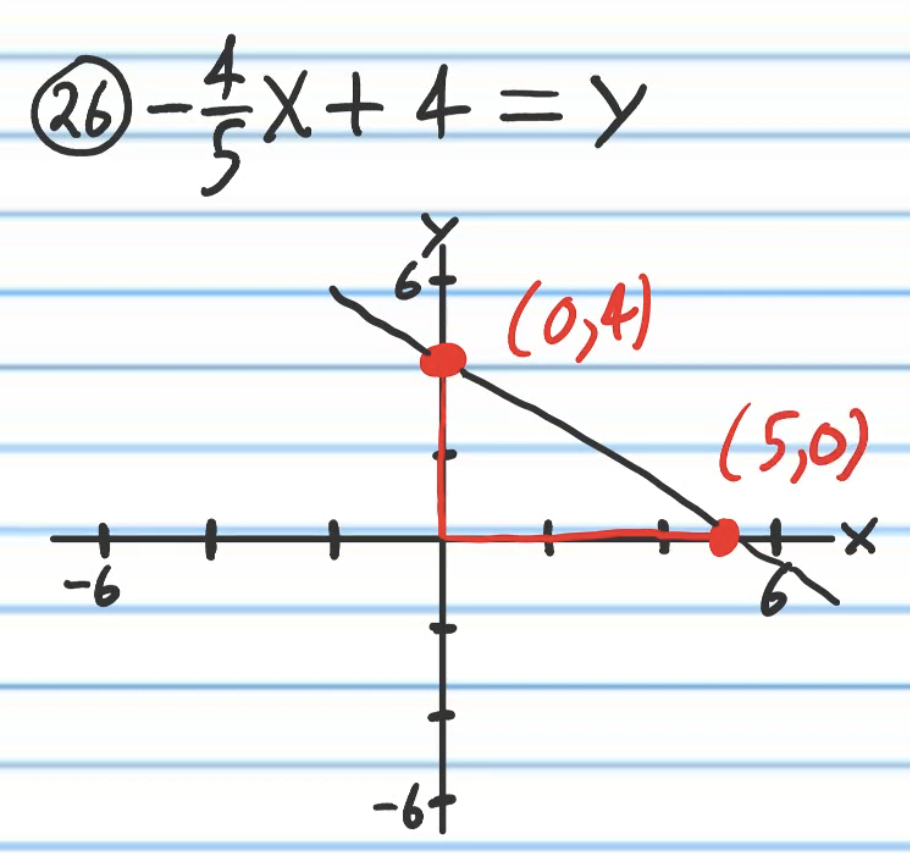
\includegraphics[width=0.5\textwidth]{beg2702.png}
  \caption{When the slope is negative}
\end{figure}

\vspace{0.5cm}

Nếu slope là whole number $2=\frac{2}{1}$. So rise 2 and run 1.

% \vspace{1cm}

Nếu rise \& run chạy ra ngoài hệ trục mình vẽ như trong hình dưới nếu rise 5 and run 3 to the right thì outside the window. Vậy mình sẽ go \textbf{down} 5 and go 3 \textbf{to the left}. Nếu gặp negative slope thì revert bằng cách go up and to the left.

\begin{figure}[htb!]
  \centering
  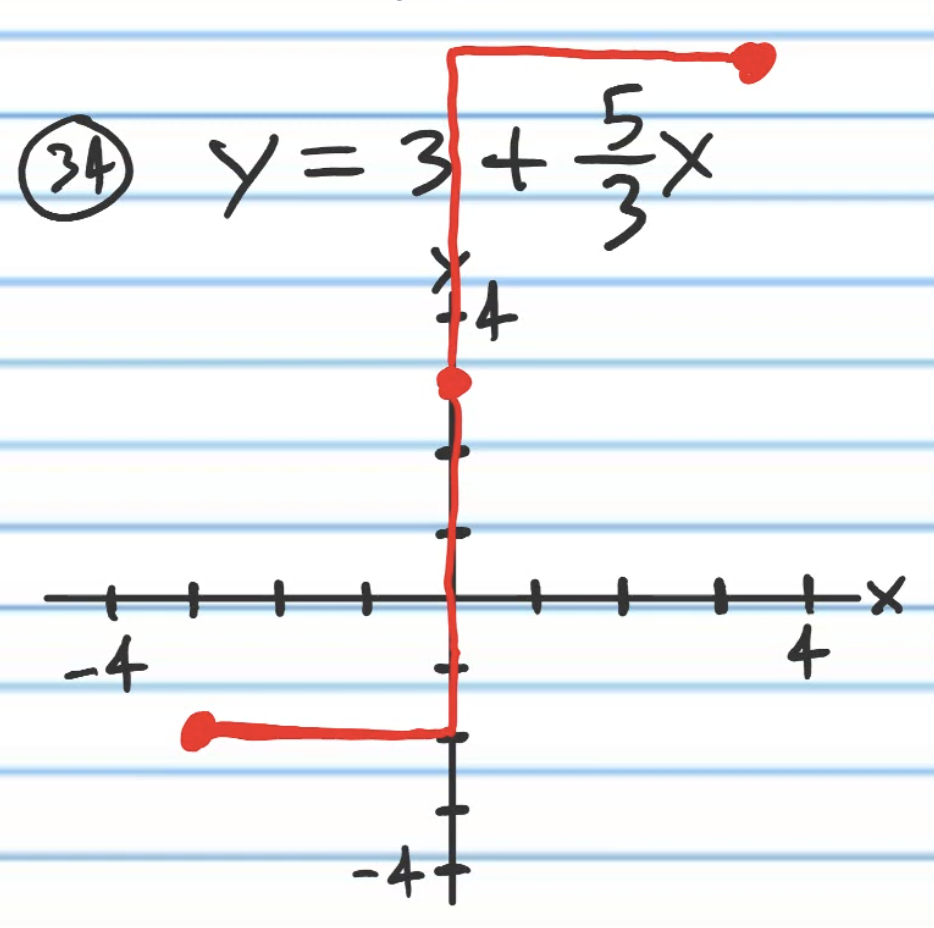
\includegraphics[width=0.5\textwidth]{beg2703.png}
  \caption{Go down and to the left}
\end{figure}

\hl{Method 04}: Using Point-Slope Form. Giống method 03.

\vspace{8mm}

In the problem below, kể cả khi revert the point thì vẫn ra ngoài our drawing window. Vậy thay vì go 3 and 4 whole units of one, we go 3 and 4 half-units of one (tức $\frac{1}{2}$) hoặc 3 and 4 third-units of one ($\frac{1}{3}$. The picture on the right go up three thirds (which is one whole $\frac{3}{3}=1$) and to the left four thirds $\frac{4}{3}$ to get to the x-coordinate $-(2+\frac{4}{3})=-3\frac{1}{3}$ (a mixed number). Chia một unit ra làm 3 phần bằng nhau. Nếu vẫn không đủ nữa thì chia ra fifths.

\begin{figure}[htb!]
  \centering
  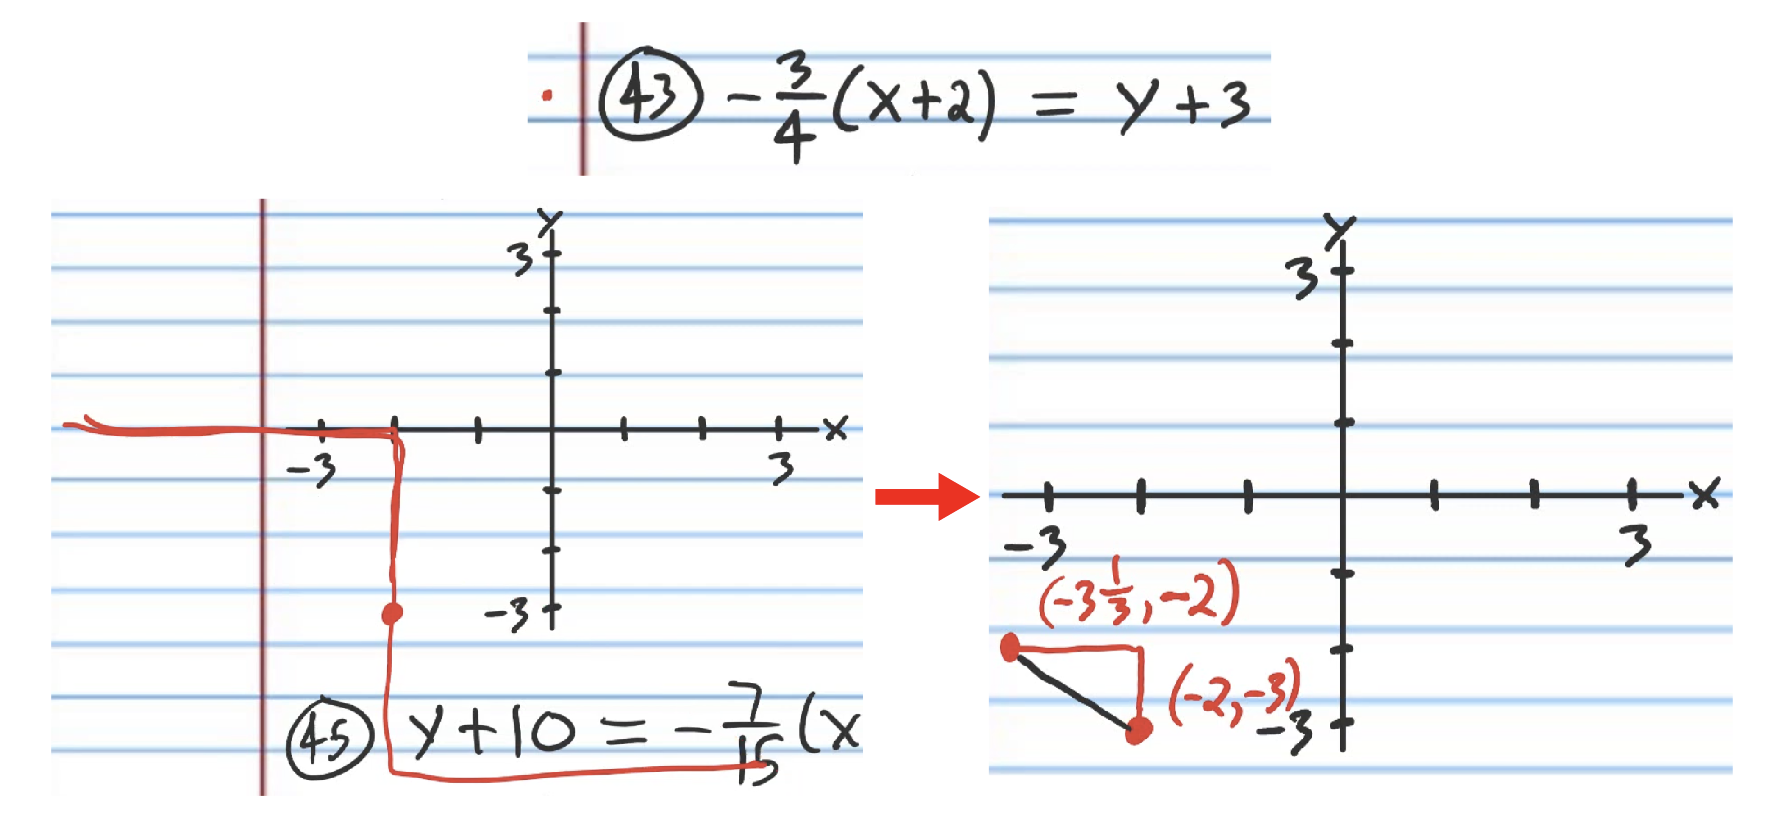
\includegraphics[width=0.9\textwidth]{beg2704.png}
  \caption{Go three thirds}
\end{figure}

\section{Additional Problems on Linear Equations and their Graphs}
% 06 Aug 2025

If two lines are parallel, their slope are equal.

If two lines are perpendicular (vuông góc), the slopes are \textbf{negative reciprocals} ($m_{2}=-(\frac{1}{m_{1}})$). Flip tử mẫu \& đổi dấu.

% Write an equation of the line shown.

\vspace{.4cm}

All Vertical lines like $x=3$ have slope of \textbf{undefined} (mẫu số có denominator chia cho zero).

All Horizontal lines like $y=1$ have slope of \textbf{zero}.

\section{Factoring Algebraic Expressions (Part I)}
%06 Sep 2025 trời chuẩn bị mưa

\begin{multicols}{2}
[
%optional header
  \textbf{Exercise}: Factor out the greatest common factor.
]

\begin{align*}
  \circled{1}\ &28x^{5}-8x^{3}+12x^{2}\\
  &=4x^{2}(7x^{3}-2x+3)
\end{align*}

\begin{align*}
  \circled{2}\ &21y^{4}-27y^{3}+15y\\
  &=3y(7y^{3}-9y^{2}+5)
\end{align*}

\begin{align*}
  \circled{3}\ &-50z^{6}+40z^{4}-15z^{3}\\
  &=-5z^{3}(10z^{3}-8z+3)
\end{align*}

\begin{align*}
  \circled{5}\ &-12y^{4}+33y^{3}-15y^{3}\\
  &=-3y^{3}(4y-11+5y^{2})
\end{align*}

\begin{align*}
  \circled{8}\ &24a^{5}b^{3}-18a^{2}-36a^{3}b^{2}\\
  &=6a^{2}(4a^{3}b^{3}-3-6ab^{2})
\end{align*}

\end{multicols}

In Problem \circled{3}, the leading term ($10z^{3}$) should be positive. Nên mình factor out the negative \& change the sign of the terms inside the parentheses.

\vspace{.6cm}

\begin{multicols}{2}
[
%optional header
  \textbf{Exercise}: Factor the quadratic expressions.
]

\begin{align*}
  \circled{15}\ &x^{2}+9x+18=(x+3)(x+5)\\
\end{align*}

  \[\circled{16}\ y^{2}+6y+5=(x+1)(x+5)\]

  \[\circled{18}\ x^{2}+8x+12=(x+2)(x+6)\]

  \[\circled{20}\ x^{2}+9x+18=(x+6)(x+3)\]

  \[\circled{26}\ z^{2}+3z-10=(z-2)(z+5)\]

  \[\circled{27}\ y^{2}-3y-28=(y-7)(y+4)\]

  \[\circled{28}\ x^{2}-15x+54=(x-6)(x-9)\]

  \[\circled{35}\ z^{2}-8z+15=(x-3)(x-5)\]

  \[\circled{29}\ z^{2}-7z-44=(z+4)(z-11)\]

  \[\circled{32}\ z^{2}+4z-21=(z+7)(z-3)\]

  \[\circled{37}\ z^{2}-12z+36=(z-6)(z-6)\]

  \[\circled{40}\ z^{2}+19z-20=(z+20)(z-1)\]

  \[\circled{42}\ x^{2}-x-12=(x+3)(x-4)\]
\end{multicols}

In Problem \circled{1}, ask yourself \q{\textbf{what two numbers multiply to 15 AND add up to 8?}} You can come up with ($1\cdot 15$) \& ($3\cdot 5$). But ($1+15=16 \neq 8$) nên chỉ còn lại 3 and 5.

Problem \circled{26} cũng làm theo cách tương tự. ($-2\cdot 5=-10$) AND ($-2+5=3$). If the last term of the trinomial is negative ($-10$), thì khi factor sẽ phải ra one positive \& one negative.

Problem \circled{28}, ta thấy last term is positive (54) but the second term is negtive ($-15x)$. Vậy khi factor phải ra 2 số âm.
